\documentclass[12pt,twoside]{article}

\textwidth 17cm \textheight 25cm \evensidemargin 0cm
\oddsidemargin 0cm \topmargin -2.5cm
\parindent 0pt
%\parskip \bigskipamount

\usepackage{graphicx}
\usepackage[dutch]{babel}
\usepackage{amssymb,amsthm,amsmath}
\usepackage[utf8]{inputenc}
\usepackage{nopageno}
\usepackage{pdfpages}
\usepackage{enumerate}
\usepackage{caption}
\usepackage{wrapfig}
\usepackage{pgf,tikz}
\usepackage{color}
\usetikzlibrary{arrows}
\usetikzlibrary{patterns}
\usepackage{fancyhdr}
\pagestyle{fancy}
\usepackage[version=3]{mhchem}
\usepackage{multicol}
\usepackage{fix-cm}
\usepackage{setspace}
\usepackage{mhchem}
\usepackage{xhfill}
\usepackage{parskip}
\usepackage{cancel}
\usepackage{mdframed}
\usepackage{url}

\newcommand{\todo}[1]{{\color{red} TODO: #1}}

\newcommand{\degree}{\ensuremath{^\circ}}
\newcommand\rad{\qopname\relax o{\mathrm{rad}}}

\newcommand\ggd{\qopname\relax o{\mathrm{ggd}}}

\def\LRA{\Leftrightarrow}%\mkern40mu}

\newcommand{\zrmbox}{\framebox{\phantom{EXE}}\phantom{X}}
\newcommand{\zrm}[1]{\framebox{#1}}

% environment oefening:
% houdt een teller bij die de oefeningen nummert, probeert ook de oefening op één pagina te houden
\newcounter{noefening}
\setcounter{noefening}{0}
\newenvironment{oefening}
{
  \stepcounter{noefening}
  \pagebreak[0]
  \begin{minipage}{\textwidth}
  \vspace*{0.7cm}{\large\bf Oefening \arabic{noefening}}
}{%
  \end{minipage}
}

\usepackage{calc}

% vraag
\reversemarginpar
\newcounter{punten}
\setcounter{punten}{0}
\newcounter{nvraag}
\setcounter{nvraag}{1}
\newlength{\puntwidth}
\newlength{\boxwidth}
\newcommand{\vraag}[1]{
\settowidth{\puntwidth}{\Large{#1}}
\setlength{\boxwidth}{1.5cm}
\addtolength{\boxwidth}{-\puntwidth}
{\large\bf Vraag \arabic{nvraag} \addtocounter{nvraag}{1}}\vspace*{-0.5cm}
{\marginpar{\color{lightgray}\fbox{\parbox{1.5cm}{\vspace*{1cm}\hspace*{\boxwidth}{\Large{#1}}}}}
\vspace*{0.5cm}}
\addtocounter{punten}{#1}}

% arulefill
\newcommand\arulefill[1][]{
  \ifstrempty{#1}{
    \leavevmode{
      \xrfill[-5pt]{0.3pt}[lightgray]
      \endgraf
    }
    \vspace*{0.2cm}
  }{
    \leavevmode{
      \xrfill[-5pt]{0.3pt}[lightgray]
      \endgraf
      \vspace*{0.2cm}
    }
    \foreach \n in {1,...,#1}{
      \leavevmode{
        \xrfill[-5pt]{0.3pt}[lightgray]
        \endgraf
        \vspace*{0.2cm}
      }
    }
  }
}
% \arules{n}
\newcommand{\arules}[1]{
\mbox{}
\color{lightgray}
%\vspace*{0.05cm}
\foreach \n in {1,...,#1}{
  \vspace*{0.75cm}
  \hrule height 0.3pt\hfill
}\color{black}\vspace*{0.2cm}}

% \arule{x}
\newcommand{\arule}[1]{
\color{lightgray}{\raisebox{-0.1cm}{\rule[-0.05cm]{#1}{0.3pt}}}\color{black}
}

% \abox{y}
\newcommand{\abox}[1]{
\fbox{
\begin{minipage}{\textwidth- 4\fboxsep}
\hspace*{\textwidth}\vspace{#1}
\end{minipage}
}
}

\newcommand{\ruitjes}[1]{
\definecolor{cqcqcq}{rgb}{0.85,0.85,0.85}
\hspace*{-2.5cm}
\begin{tikzpicture}[scale=1.04,line cap=round,line join=round,>=triangle 45,x=1.0cm,y=1.0cm]
\draw [color=cqcqcq, xstep=0.5cm, ystep=0.5cm] (0,-#1) grid (20.5,0);
\end{tikzpicture}
}


\newcommand{\assenstelsel}[5][1]{
\definecolor{cqcqcq}{rgb}{0.65,0.65,0.65}
\begin{tikzpicture}[scale=#1,line cap=round,line join=round,>=triangle 45,x=1.0cm,y=1.0cm]
\draw [color=cqcqcq,dash pattern=on 1pt off 1pt, xstep=1.0cm,ystep=1.0cm] (#2,#4) grid (#3,#5);
\draw[->,color=black] (#2,0) -- (#3,0);
\draw[shift={(1,0)},color=black] (0pt,2pt) -- (0pt,-2pt) node[below] {\footnotesize $1$};
\draw[color=black] (#3.25,0.07) node [anchor=south west] { x};
\draw[->,color=black] (0,#4) -- (0,#5);
\draw[shift={(0,1)},color=black] (2pt,0pt) -- (-2pt,0pt) node[left] {\footnotesize $1$};
\draw[color=black] (0.09,#5.25) node [anchor=west] { y};
\draw[color=black] (0pt,-10pt) node[right] {\footnotesize $0$};
\end{tikzpicture}
}

\newcommand{\getallenas}[3][1]{
\definecolor{cqcqcq}{rgb}{0.65,0.65,0.65}
\begin{tikzpicture}[scale=#1,line cap=round,line join=round,>=triangle 45,x=1.0cm,y=1.0cm]
\draw [color=cqcqcq,dash pattern=on 1pt off 1pt, xstep=1.0cm,ystep=1.0cm] (#2,-0.2) grid (#3,0.2);
\draw[->,color=black] (#2.25,0) -- (#3.5,0);
\draw[shift={(0,0)},color=black] (0pt,2pt) -- (0pt,-2pt) node[below] {\footnotesize $0$};
\draw[shift={(1,0)},color=black] (0pt,2pt) -- (0pt,-2pt) node[below] {\footnotesize $1$};
\draw[color=black] (#3.25,0.07) node [anchor=south west] {$\mathbb{R}$};
\end{tikzpicture}
}

\newcommand{\visgraad}[1]{\begin{tabular}{p{0.5cm}|p{#1}}&\\\hline\\\end{tabular}}

\newcommand{\tekenschema}[2]{\begin{tabular}{p{0.5cm}|p{#1}}&\\\hline\\[#2]\end{tabular}}

% schema van Horner
\newcommand{\schemahorner}{
\begin{tabular}{p{0.5cm}|p{7cm}}
&\\[1.5cm]
\hline\\
\end{tabular}}

% geef tabular iets meer ruimte
\setlength{\tabcolsep}{14pt}
\renewcommand{\arraystretch}{1.5}

\newcommand{\toets}[3]{
\thispagestyle{plain}
\vspace*{-2.5cm}
\begin{tikzpicture}[remember picture, overlay]
    \node [shift={(15.25 cm,-1.6cm)}] {%
        \includegraphics[width=1.8cm]{/home/ppareit/kaa1415/logokaavelgem.png}%
    };%
\end{tikzpicture}

\begin{tabular}{|llc|c|}
\hline
\vspace*{-0.5cm}
&&&\\
Naam & \arule{4cm} & {\Large\bf KA AVELGEM} & \\
\vspace*{-0.75cm}
&&&\\
Klas & \arule{4cm} & {\Large\bf 20...-...-...} & \\
\hline
\vspace*{-0.75cm}
&&&\\
Toets & {\bf #2} & {\large\bf #1} & Beoordeling\\
\vspace*{-0.75cm}
&&&\\
Onderwerp & \multicolumn{2}{l|}{\bf #3} &\\
\hline
\end{tabular}
}

\newcommand{\oefeningen}[1]{

\fancyhead[LE, RO]{\vspace{0.5cm} #1}
%\thispagestyle{plain}

{\bf \Large \centering Oefeningen: #1}

}

\raggedbottom

\newcommand\dom{\qopname\relax o{\mathrm{dom}}}
\newcommand\ber{\qopname\relax o{\mathrm{ber}}}

\newcommand\mC{\qopname\relax o{\mathrm{mC}}}
\newcommand\uC{\qopname\relax o{\mathrm{{\mu}C}}}
\newcommand\C{\qopname\relax o{\mathrm{C}}}

\newcommand\W{\qopname\relax o{\mathrm{W}}}
\newcommand\kW{\qopname\relax o{\mathrm{kW}}}
\newcommand\kWh{\qopname\relax o{\mathrm{kWh}}}


\newcommand\V{\qopname\relax o{\mathrm{V}}}
\newcommand\ohm{\qopname\relax o{\mathrm{\Omega}}}
\newcommand\kohm{\qopname\relax o{\mathrm{k\Omega}}}


\newcommand\N{\qopname\relax o{\mathrm{N}}}

\newcommand\Nperkg{\qopname\relax o{\mathrm{N/kg}}}

\newcommand\Nperm{\qopname\relax o{\mathrm{N/m}}}

\newcommand\gpermol{\qopname\relax o{\mathrm{g/mol}}}


\newcommand\kgperm{\qopname\relax o{\mathrm{kg/m}}}
\newcommand\kgperdm{\qopname\relax o{\mathrm{kg/dm}}}
\newcommand\gpercm{\qopname\relax o{\mathrm{g/cm}}}
\newcommand\gperml{\qopname\relax o{\mathrm{g/ml}}}


\newcommand{\mA}{\;\mbox{mA}}
\newcommand{\A}{\;\mbox{A}}
\newcommand{\MA}{\;\mbox{MA}}

\newcommand{\us}{\;\mu\mbox{s}}
\newcommand\s{\qopname\relax o{\mathrm{s}}}

\newcommand\h{\qopname\relax o{\mathrm{h}}}

\newcommand{\mpers}{\;\mbox{m/s}}
\newcommand{\kmperh}{\;\mbox{km/h}}
\newcommand{\kmpermin}{\;\mbox{km/min}}
\newcommand{\kmpers}{\;\mbox{km/s}}

\newcommand{\mph}{\;\mbox{mph}}

\newcommand{\Hz}{\;\mbox{Hz}}

\newcommand\Gm{\qopname\relax o{\mathrm{Gm}}}
\newcommand\Mm{\qopname\relax o{\mathrm{Mm}}}
\newcommand\km{\qopname\relax o{\mathrm{km}}}
\newcommand\hm{\qopname\relax o{\mathrm{hm}}}
\newcommand\dam{\qopname\relax o{\mathrm{dam}}}
\newcommand\m{\qopname\relax o{\mathrm{m}}}
\newcommand\dm{\qopname\relax o{\mathrm{dm}}}
\newcommand\cm{\qopname\relax o{\mathrm{cm}}}
\newcommand\mm{\qopname\relax o{\mathrm{mm}}}
\newcommand\um{\qopname\relax o{\mathrm{{\mu}m}}}
\newcommand\nm{\qopname\relax o{\mathrm{nm}}}


\newcommand\Gg{\qopname\relax o{\mathrm{Gg}}}
\newcommand\Mg{\qopname\relax o{\mathrm{Mg}}}
\newcommand\kg{\qopname\relax o{\mathrm{kg}}}
\newcommand\hg{\qopname\relax o{\mathrm{hg}}}
\renewcommand\dag{\qopname\relax o{\mathrm{dag}}}
\newcommand\g{\qopname\relax o{\mathrm{g}}}
\newcommand\dg{\qopname\relax o{\mathrm{dg}}}
\newcommand\cg{\qopname\relax o{\mathrm{cg}}}
\newcommand\mg{\qopname\relax o{\mathrm{mg}}}
\newcommand\ug{\qopname\relax o{\mathrm{{\mu}g}}}
\renewcommand\ng{\qopname\relax o{\mathrm{ng}}}

\newcommand\ton{\qopname\relax o{\mathrm{ton}}}

\newcommand\Gl{\qopname\relax o{\mathrm{Gl}}}
\newcommand\Ml{\qopname\relax o{\mathrm{Ml}}}
\newcommand\kl{\qopname\relax o{\mathrm{kl}}}
\newcommand\hl{\qopname\relax o{\mathrm{hl}}}
\newcommand\dal{\qopname\relax o{\mathrm{dal}}}
\renewcommand\l{\qopname\relax o{\mathrm{l}}}
\newcommand\dl{\qopname\relax o{\mathrm{dl}}}
\newcommand\cl{\qopname\relax o{\mathrm{cl}}}
\newcommand\ml{\qopname\relax o{\mathrm{ml}}}
\newcommand\ul{\qopname\relax o{\mathrm{{\mu}l}}}
\newcommand\nl{\qopname\relax o{\mathrm{nl}}}

\newcommand\MJ{\qopname\relax o{\mathrm{MJ}}}
\newcommand\kJ{\qopname\relax o{\mathrm{kJ}}}
\newcommand\J{\qopname\relax o{\mathrm{J}}}

\newcommand\T{\qopname\relax o{\mathrm{T}}}
\newcommand\uT{\qopname\relax o{\mathrm{{\mu}T}}}

\newcommand\grC{\qopname\relax o{\mathrm{{\degree}C}}}

\newcommand\K{\qopname\relax o{\mathrm{K}}}
\newcommand\calperK{\qopname\relax o{\mathrm{cal/K}}}

\newcommand\hPa{\qopname\relax o{\mathrm{hPa}}}
\newcommand\Pa{\qopname\relax o{\mathrm{Pa}}}

\newcommand\dB{\qopname\relax o{\mathrm{dB}}}

\newcommand{\EE}[1]{\cdot 10^{#1}}

\onehalfspacing

%\singlespacing
%\onehalfspacing
%\doublespacing

%\setlength{\headsep}{0cm}

\newenvironment{exlist}[1] %
{ \begin{multicols}{#1}
  \begin{enumerate}[(a)]
    \setlength{\itemsep}{0.8em} }
{ \end{enumerate}
  \end{multicols} }




\usepackage{pgfplots}

\usepackage{relsize}

\begin{document}

\thispagestyle{empty}
\begin{center}
  \begin{mdframed}
  \centering
  \fontsize{40}{60}\selectfont Exponentiële functies
  \end{mdframed}
  \vfill
\begin{tikzpicture}[line cap=round,line join=round,>=triangle 45,x=1.0cm,y=1.0cm]
\draw[->,color=black] (-2.52,0) -- (6.4,0);
\foreach \x in {-2,2,4,6}
\draw[shift={(\x,0)},color=black] (0pt,2pt) -- (0pt,-2pt) node[below] {\footnotesize $\x$};
\draw[->,color=black] (0,-1.22) -- (0,4.36);
\foreach \y in {,2,4}
\draw[shift={(0,\y)},color=black] (2pt,0pt) -- (-2pt,0pt) node[left] {\footnotesize $\y$};
\draw[color=black] (0pt,-10pt) node[right] {\footnotesize $0$};
\clip(-2.52,-1.22) rectangle (6.4,4.36);
\draw[line width=1.6pt,dash pattern=on 3pt off 4pt, smooth,samples=50,domain=-2.5:6.4] plot(\x,{(\x)});
\draw[line width=1.6pt, smooth,samples=100,domain=-2.5:2.4] plot(\x,{exp(\x)});
\draw[line width=1.6pt, smooth,samples=100,domain=0.1:6.4] plot(\x,{ln((\x))});
\draw (1.26,3.98) node[anchor=north west] {$f(x)=e^x$};
\draw (3.5,1.3) node[anchor=north west] {$f^{-1}(x)=\ln(x)$};
\end{tikzpicture}
%  \includegraphics[width=0.8\textwidth]{}
  \vfill
\end{center}

\subsection*{Doelstellingen}
\vspace*{-0.8cm}
{\singlespacing
Je \hfill  {\scriptsize(LP2005-069, LI1.5, ET10-11-13)}
\begin{itemize}
  \itemsep-0.2em
  \item kent de definitie van een macht met een negatieve exponent.
  \item kan de elementaire rekenregels toepassen bij machten met negatieve exponenten.
  \item kan $n$-de wortels berekenen in $\mathbb{R}$.
  \item kent de definitie van een macht met een rationale exponent.
  \item kan de elementaire rekenregels toepassen bij machten met rationale exponenten.
  \item kent het begrip logaritme met grondtal 10.
  \item kan de volgende rekenregels toepassen: logaritme van een product, logaritme van een quotiënt en logaritme van een macht.
  \item kan de grafieken van de lineaire functie $f(x) = ax + b$ en de exponentiële functie $f(x) = b\cdot a^x$ opstellen met behulp van een tabel en hierbij het onderscheid maken tussen lineaire en exponentiële groei.
  \item kan van de grafiek van exponentiële functies $f(x)=b\cdot a^x$ het stijgen/dalen, de limietwaarden en
het asymptotisch gedrag aflezen.
  \item kan problemen van groeitoepassingen met gegeven functioneel verband oplossen met behulp van ICT en deze oplossing interpreteren.
\end{itemize}}
\subsection*{Vaardigheden en attitudes}
\vspace*{-0.8cm}
{\singlespacing
Je \hfill {\scriptsize(LP2005-069, ET2-3-6)}
\begin{itemize}
  \itemsep-0.2em
  \item maakt gebruik van wiskundige technieken zoals figuren maken en tabellen opstellen.
  \item maakt functioneel gebruik van ICT bij het oplossen van problemen.
  \item verantwoordt keuzes m.b.t. representatie en gevolgde werkwijze.
\end{itemize}
}
\vspace*{-1cm}

\thispagestyle{empty}
\mbox{}
\newpage
\clearpage
\thispagestyle{empty}
\mbox{}
\newpage
\clearpage
\pagenumbering{arabic} 

\fancyhead[RO,LE]{Exponentiële functies}
\fancyhead[RE,LO]{}


\section{Machten met natuurlijke exponenten}

Herinner je nog de definitie voor een macht met een reëel grondtal en een natuurlijke exponent:

\paragraph*{Definitie}

\begin{mdframed}
\begin{align*}
\forall a \in \mathbb{R}, \forall n\in \mathbb{N}\setminus\{0,1\} : a^n &= \underbrace{a\cdot a\cdot a \ldots \cdot a}_{\mbox{$n$ factoren}}\\
a^1 &= a\\
\forall a \in \mathbb{R}_0 : a^0 &= 1
\end{align*}
\end{mdframed}

\begin{oefening}
In de bovenstaande definitie moet $n\in \mathbb{N}\setminus\{0,1\}$, geef de mogelijke waarden voor $n$.
\arules{1}
\end{oefening}

\begin{oefening}
Bereken m.b.v. de definitie:\\
\begin{enumerate}[(a)]
  \itemsep1em
  \item $3^4=$\arulefill
  \item $(-2)^4=$\arulefill
  \item $-3^2=$\arulefill
  \item $91^1=$\arulefill
  \item $\left(321^4\right)^0=$\arulefill
\end{enumerate}
\end{oefening}

\begin{oefening}
Waarom mag in de laatste regel van de definitie $a$ geen $0$ zijn?
\end{oefening}

\begin{oefening}
Geef de tekenregels voor machten:
\arules{4}
\end{oefening}

\section{Machten met negatieve gehele exponenten}

Vroeger definieerden we reeds machten met negatieve gehele exponenten:
\paragraph*{Definitie}
\begin{mdframed}
\begin{align*}
\forall a \in \mathbb{R}_0, \forall n\in \mathbb{N}: a^{-n} = \left(a^{-1}\right)^n=\left(a^n\right)=\dfrac{1}{a^n}
\end{align*}
\end{mdframed}

\begin{oefening}
Bereken:
\begin{enumerate}[(a)]
  \itemsep1em
  \item $3^{-4}=$\arulefill
  \item $(-2)^{-4}=$\arulefill
  \item $-3^{-2}=$\arulefill
  \item $91^{-1}=$\arulefill
  \item $\left(\dfrac{1}{3}\right)^{-3}=$\arulefill
  \item $\dfrac{1^{-5}}{2}=$\arulefill
  \item $\dfrac{1}{5^{-2}}=$\arulefill
\end{enumerate}
\end{oefening}

De rekenregels die gelden voor natuurlijke exponenten blijven gelden voor machten met gehele exponenten.

\paragraph*{Rekenregels voor machten met gehele exponenten}
\begin{mdframed}
$\forall a, b, c \in \mathbb{R}_0, \forall m, n\in \mathbb{Z}:$
\begin{align*}
a^m\cdot a^n &= a^{m+n} && \mbox{machten met zelfde grondtal vermenigvuldigen}\\
\dfrac{a^m}{a^n} &= a^{m-n} && \mbox{machten met zelfde grondtal delen}\\
\left(a^m\right)^n &= a^{m\cdot n} && \mbox{macht van een macht}\\
\left(abc\right)^m &= a^mb^mc^m && \mbox{product tot een macht}\\
\left(\dfrac{a}{b}\right)^m &= \dfrac{a^m}{b^m} && \mbox{quotiënt tot een macht}\\
\end{align*}
\end{mdframed}

\begin{oefening}
Begrijp je in bovenstaande definitie de gekozen benamingen?
\end{oefening}

\begin{oefening}
Bereken, maak steeds gebruik van één of meer van bovenstaande rekenregels:
\begin{enumerate}[(a)]
  \itemsep1em
  \item $2^{-3}\cdot2^5=$\arulefill
  \item $2\cdot 2^2=$\arulefill
  \item $\dfrac{(-2)^3}{(-2)^2}=$\arulefill
  \item $\dfrac{103^{-2}\cdot 103}{103^{-1}}=$\arulefill
  \item $\dfrac{8^2}{2^5}=$\arulefill\mbox{hint: schrijf eerst 8 als een macht met grondtal 2}
  \item $\dfrac{\left(3\cdot4\right)^8}{3^6\cdot 2^{16}}=$\arulefill
  \item $\dfrac{49^2}{7^2}=$\arulefill
\end{enumerate}
\end{oefening}

\begin{oefening}
Kan je zelf een rekenregel afleiden voor de macht van een quotiënt met negatieve exponent?
\arules{3}
\end{oefening}

% Extra oefeningen:
% Hoe leg je aan iemand die regels niet kent, uit dat $a^3\cdot a^4 = a^7$? En dat $(a^3)^4= a^12$?
% Leg uit dat de afspraak $a^0 = 1$ in overeenstemming is met de regel {\em machten met zelfde grondtal delen}

\begin{oefening}
Bereken en controleer nadien met het \zrm{ZRM}.
\begin{multicols}{4}
\begin{enumerate}[(a)]
  \itemsep1em
  \item $\left(-3\right)^0$
  \item $\left(-4\right)^1$
  \item $\left(\dfrac{1}{3}\right)^5:\dfrac{1}{3}$
  \item $\left(\dfrac{4}{5}\right)^{-1}$
  \item $\left(-\dfrac{1}{6}\right)^{-3}$
  \item $\left(\dfrac{2}{5}\right)^{-2}$
  \item $2^{-1}$
  \item $\left(-\dfrac{2}{5}\right)^{-2}$
  \item $\left[\left(-1\right)^6\right]^3$
  \item $[-1^6]^3$
  \item $\dfrac{0.8^{-3}}{0.8^{-6}}$
  \item $\dfrac{\left(-4\right)^{0}}{\left(-4\right)^{-2}}$
  \item $[\left(-0.1\right)^2]^3$
  \item $\left(\sqrt{2}\right)^{-2}$
  \item $1.1^2$
  \item $0.3^{-2}$
  \item $\left(-0.01\right)^{-5}$
  \item $\left(-0.05\right)^{-1}$
  \item $0.2^{-4}$
  \item $0.08^{-3}$
  \item $0.5^{-2}\cdot0.5^{-3}$
  \item $\left(-2\cdot2^{-2}\right)^{-2}$
  \item $\dfrac{1}{\left(\sqrt{2}\right)}^{-2}$
\end{enumerate}
\end{multicols}
\end{oefening}

\begin{oefening}
Bereken volgende machten zonder \zrm{ZRM}. Maak steeds een tussenstap.
\begin{multicols}{3}
  \begin{enumerate}[(a)]
    \itemsep1em
    \item $-(-2)^3$
    \item $-(-3)^2$
    \item $-2^{-3}$
    \item $3^{-2}$
    \item $(-2)^{-4}$
    \item $(-2)^{-5}$
    \item $(-1)^{802}$
    \item $-(-604)^{0}$
    \item $\left(-\dfrac{\sqrt{7}}{8\pi}\right)^{0}$
    \item $2.5^{2}$
    \item $0.04^{3}$
    \item $\left(-\dfrac{6}{11}\right)^{2}$
    \item $\left(-\dfrac{4}{5}\right)^{3}$
    \item $\left(-\dfrac{1}{3}\right)^{-3}$
    \item $\left(\dfrac{2}{7}\right)^{-2}$
    \item $\left(\sqrt{2}\right)^{2}$
    \item $\left(\sqrt{2}\right)^{4}$
    \item $\left(\sqrt{2}\right)^{-1}$
    \item $(-0.01)^{-4}$
    \item $\left(-\dfrac{1}{\sqrt{5}}\right)^{1}$
    \item $\left(-\dfrac{5}{\sqrt{2}}\right)^{-2}$
    \item $\left(\dfrac{\sqrt{2}}{3}\right)^{-4}$
    \item $\left(-\dfrac{1}{\sqrt{3}}\right)^{-6}$
    \item $\left(-\dfrac{45}{60}\right)^{3}$
    \item $(1.5)^{-2}$
    \item $\dfrac{1}{4^{-2}}$
  \end{enumerate}
\end{multicols}
\end{oefening}

\begin{oefening}
Vereenvoudig:
\begin{multicols}{3}
  \begin{enumerate}[(a)]
  \itemsep1em
  \item $a^2\cdot a^3$
  \item $a^2+a^3$
  \item $a^9\cdot2^{-5}$
  \item $\dfrac{a^8}{\left({a^2}\right)^4}$
  \item $\left(a^8\right)^2$
  \item $\left(\dfrac{a^2}{b^4}\right)^{-2}$
  \item $a^2\cdot a^8$
  \item $a^4\cdot a^{-2}$
  \item $x^2\cdot y^2$
  \item $a^2b^3c^4a^{-2}b^{-3}c^{-4}$
  \item $a^2a^2-a^4$
  \item $\dfrac{a^0}{b^0}$
  \item $\dfrac{a^1}{b^2}$
  \item $a^2+a^2$
  \item $a^2+a^3$
  \item $\dfrac{a^3}{a^2}$
  \item $\dfrac{a^{-10}}{a^{-5}}\cdot{a^3}$
  \item $\dfrac{x^2y^1z^0}{x^{-2}y^{-1}z^{0}}$
  \item $4^a+2^{2a}$
  \item $4^a\cdot2^{2a}$
  \item $\frac{2a\cdot a^{2}}{a^{3}}$
  \item $\left(-a^4\right)\cdot\left(+a^4\right)$
  \item $\left(-a^4\right):\left(+a^4\right)$
  \item $\left(-0.5ab^2\right)^3$
  \item $\left(\left(xy\right)^4y\right)^{-2}$
  \item $\left(\dfrac{2a}{b^{-2}}\right)^2$
\end{enumerate}
\end{multicols}
\end{oefening}

\begin{oefening}
Werk uit:
\begin{multicols}{4}
  \begin{enumerate}[(a)]
    \itemsep1em
    \item $2^3\cdot 2^2$
    \item $10^4\cdot 10^2$
    \item $\left(\dfrac{2}{3}\right)\cdot \left(\dfrac{2}{3}\right)^2$
    \item $2^8\cdot 2^{-6}$
    \item $\left(-2\right)^4\cdot \left(-2\right)^{-4}$
    \item $\left(-\frac{1}{2}\right)^{-4}\cdot \left(-\frac{1}{2}\right)^2$
    \item $8^4\cdot 8\cdot 8^{-6}$
    \item $0.3\cdot 0.3^5\cdot 0.3^{-3}$
    \item $2^5: 2^2$
    \item $10^3: 10^2$
    \item $\left(\dfrac{3}{4}\right)^3: \left(\dfrac{3}{4}\right)$
    \item $3^{-2}: 3^3$
    \item $\dfrac{10^{-1}}{10^{-3}}$
    \item $\dfrac{2^{3}}{2^{7}}$
    \item $\dfrac{(-2)^{-5}}{(-2)^{-2}}$
    \item $3.2^{-1}:3.2^{-3}$
    \item $6^2\cdot 6^{-3}$
    \item $\dfrac{9^4}{9^2}$
    \item $\left(-3\right)^{-1}\cdot \left(-3\right)^3$
    \item $\dfrac{\left(-1\right)^{-4}}{\left(-1\right)^{-1}}$
    \item $4^3\cdot 4^{-6}$
    \item $\dfrac{\left(-5\right)^{-3}}{\left(-5\right)^{-1}}$
    \item $10^3\cdot 10^{-3}$
    \item $\dfrac{-3^3}{3^4}$
    \item $1^4\cdot1\cdot1^{-6}$
    \item $\dfrac{\left(-3\right)^{2}}{\left(-3\right)^{4}}$
%    \item $10^2-1^2$
%    \item $\left(-1\right)^6\cdot \left(-1\right)^{-3}$
%    \item $\dfrac{7^{3}}{7^{5}}$
%    \item $\left(-5\right)^4\cdot \left(-5\right)^{-2}$
%    \item $\dfrac{1.4^{-3}}{1.4^{-2}}$
%    \item $\left(-2\right)^4\cdot \left(-2\right)^{-6}$
  \end{enumerate}
\end{multicols}
\end{oefening}

\begin{oefening}
Noteer korter, indien mogelijk.
\begin{multicols}{3}
  \begin{enumerate}[(a)]
    \itemsep1em
    \item $x\cdot x\cdot x$
    \item $x+x+x$
    \item $a^5\cdot a^2$
    \item $b^7\cdot b^3\cdot b^8$
    \item $\left(-x^2\right)\left(-x^2\right)$
    \item $-x^2-x^2-x^2$
    \item $a\cdot a^6$
    \item $\left(x^5\right)^2$
    \item $\left(a^3\right)^3$
    \item $\left(-x^3\right)^2$
    \item $\left(x^2\right)^3$
    \item $a^8\cdot a^{-4}$
    \item $\left(-a^{-2}\right)^3$
    \item $a^4+a^4$
    \item $\left(a^4\right)^2\left(a^3\right)^5$
    \item $a^2\left(a^7\right)^3\left(a^4\right)^2$
    \item $ab^2+ab^2+ab^2$
    \item $ab^2\cdot ab^2\cdot ab^2$
    \item $\left(-x^3\right)^2\left(-x^2\right)^3$
    \item $\left(abc\right)^2\left(2bc\right)^3$
    \item $a^{-3}\cdot a$
%    \item $\left(5a\right)^{-2}$
%    \item $\left(\dfrac{-3}{y}\right)^{-3}$
%    \item $\dfrac{\left(6a^3\right)^2}{\left(-3a\right)^3}$
%    \item $ab^-2:bz^-2$
  \end{enumerate}
\end{multicols}
\end{oefening}

\begin{oefening}
Werk zo ver mogelijk uit en schrijf de uitkomst steeds met een positieve exponent.
\begin{multicols}{4}
  \begin{enumerate}[(a)]
    \itemsep1em
    \item $\left(2a\right)^{4}$
    \item $\left(-2b\right)^{3}$
    \item $\left(-ax\right)\cdot\left(-ax\right)^{2}$
    \item $\left(-x^2y^3\right)^{2}$
    \item $2a^2\cdot 4a^3$
    \item $\left(-4a\cdot 2b\right)^2$
    \item $x^3\cdot\left(-2x\right)^2$
    \item $\left(-2x^{-3}\right)^0$
    \item $\left(-x^3\right)^2$
    \item $\left(\dfrac{3a}{2b}\right)^{-1}$
    \item $\left(a^{-2}\right)^{-3}$
    \item $\left(-3x^2\right)^3$
%    \item $\left(2x\right)^3:\left(2x\right)^2$
%    \item $-3a\cdot4a^2\cdot a^{-1}$
%    \item $\left(-a\right)^3:\left(+a\right)^3$
%    \item $\left(2a\right)^{-2}$
%    \item $\dfrac{x^2\cdot x^3}{x^4}$
%    \item $\left(a^2\right)^{-3}$
%    \item $\left[\left(-2\right)^{-2}\right]^{2}$
%    \item $\left(-4a\right)^{-2}$
%    \item $\left(\dfrac{1}{3x}\right)^{-4}$
%    \item $\left[\left(-\dfrac{1}{3}\right)^{-2}\right]^{-1}$
%    \item $\left(a^0\right)^{-2}$
%    \item $\dfrac{a^2\cdot a^2\cdot a^2}{a\cdot a\cdot a}$
%    \item $\left(a^3\right)^4:a^4$
%    \item $\left(-3b\right)^{-1}$
%    \item $\left(-3b^2\right)^{-2}$
%    \item $\left(\dfrac{1}{2a^2b}\right)^{-3}$
  \end{enumerate}
\end{multicols}
\end{oefening}


\pagebreak
\section{Machtswortels}

\paragraph*{Definitie}
\begin{mdframed}
Indien $a$ een reëel getal is en $n$ een natuurlijk getal is verschillend van nul, dan is $x$ een {\bf n-de machtswortel} uit $a$ als
$$x^n=a$$
\end{mdframed}

\begin{oefening}
$-8$ en $8$ zijn de 2-de machtswortels uit $64$, waarom?
\arules{2}
\end{oefening}

\begin{oefening}
Geef alle $3$-de machtswortels uit $-64$ en zeg waarom het $3$-de machtswortels zijn.
\arules{2}
\end{oefening}

\begin{oefening}
Hoeveel $2$-de machtswortels heeft $-64$?
\arules{2}
\end{oefening}

\paragraph*{Aantal $n$-de machtswortels}
\begin{mdframed}
\begin{itemize}
  \item Indien $n$ even is en $a\geq 0$, dan heeft $a$ twee $n$-de machtswortels die tegengesteld zijn. De positieve $n$-de machtswortel wordt genoteerd als $\sqrt[n]{a}$, de negatieve als $-\sqrt[n]{a}$.
  \item Indien $n$ even is en $a < 0$, dan heeft $a$ geen $n$-de machtswortels.
  \item Indien $n$ oneven is, dan heeft $a$ juist één $n$-de machtswortel en wordt deze genoteerd als $\sqrt[n]{a}$.
\end{itemize}
\end{mdframed}

\begin{oefening}
Neem $n$ oneven, wat weet je dan over het teken van de $n$-de machtswortel?
\arules{4}
\end{oefening}

De positieve $2$-de machtswortel uit $a\in\mathbb{R}^+$ wordt de {\bf vierkantswortel} uit $a$ genoemd. De $n=2$ kan weg gelaten worden in de notatie van de wortel:
$$\sqrt{a}:=\sqrt[2]{a}$$

\begin{oefening}
\begin{enumerate}[(a)]
  \item Schrijf alle 4-de machtswortels op van $7$, zonder deze uit te rekenen.
        \arules{1}
  \item Schrijf alle 4-de machtswortels op van $-7$, zonder deze uit te rekenen.
        \arules{1}
  \item Schrijf alle 3-de machtswortels op van $5$, zonder deze uit te rekenen.
        \arules{1}
  \item Schrijf alle 3-de machtswortels op van $-5$, zonder deze uit te rekenen.
        \arules{1}
  \item Schrijf alle 2-de machtswortels op van $3$, zonder deze uit te rekenen.
        \arules{1}
\end{enumerate}
\end{oefening}

\begin{oefening}
Een eenvoudig trucje van een getal $a\in\mathbb{R}$ de absolute waarde te vinden is dat getal eerst kwadrateren en van het bekomen resultaat de positieve vierkantswortel te nemen. Leg uit waarom dit werkt.
$$|a| = \sqrt{a^2}$$
\end{oefening}


\paragraph*{Eigenschappen van machtswortels}
\begin{mdframed}
$\forall a, b \in\mathbb{R}\mbox{ en zodat volgende machtswortels zinvol zijn}, \forall m,n,p\in\mathbb{N}_0$
\begin{align*}
  \sqrt[n]{ab} &= \sqrt[n]{a}\sqrt[n]{b}\\
  \sqrt[n]{\dfrac{a}{b}} &= \dfrac{\sqrt[n]{a}}{\sqrt[n]{b}}\\
  \sqrt[n]{a^m} &= \left(\sqrt[n]{a}\right)^m\\
  \sqrt[n]{\sqrt[m]{a}} &= \sqrt[m\cdot n]{a}\\
  \sqrt[n\cdot p]{a^{m\cdot p}} &= \sqrt[n]{a^m}\\
  \sqrt[n]{a^n} &= a
\end{align*}
\end{mdframed}

\begin{oefening}
Werk uit, gebruik steeds één van bovenstaande eigenschappen:
\begin{enumerate}[(a)]
  \itemsep1em
  \item $\sqrt[3]{27\cdot 8}=$\arulefill
  \item $\sqrt[4]{\dfrac{64}{16}}=$\arulefill
  \item $\sqrt{4^3}=$\arulefill
  \item $\sqrt[3]{\sqrt{\pi}}=$\arulefill
  \item $\sqrt[5]{81^4\cdot 3^4}=$\arulefill
\end{enumerate}
\end{oefening}

\begin{oefening}
Werk uit en vereenvoudig:
\begin{multicols}{3}
\begin{enumerate}[(a)]
  \itemsep1em
  \item $2\sqrt[3]{8}+\sqrt[3]{8}$
  \item $\left(\sqrt{4}\right)^2$
  \item $\sqrt{32}$
  \item $\sqrt[3]{\frac{64}{125}}$
  \item $\sqrt[4]{16}$
  \item $\sqrt[3]{4}$
  \item $\left(-2\sqrt[3]{4}\right)^6$
  \item $\left(\sqrt[4]{5}\right)^8$
  \item $\sqrt{98}+\sqrt{72}-\sqrt{32}$
  \item $\sqrt{80}+\sqrt{45}-\sqrt{125}$
  \item $\left(\sqrt{27}-\sqrt{12}\right)\sqrt{3}$
  \item $\left(\sqrt{27}-\sqrt{12}\right):\sqrt{3}$
  \item $\left(\sqrt[3]{4}+\sqrt[3]{108}\right)\sqrt[3]{2}$
  \item $\left(\sqrt[3]{16}+\sqrt[3]{1024}\right)\sqrt[3]{4}$
  \item $\left(\sqrt[4]{128}+\sqrt[4]{8}\right)\sqrt[4]{2}$
  \item $\left(\sqrt{7}+2\right)\left(\sqrt{7}-2\right)$
  \item $\left(\sqrt{40}-\sqrt{10}\right)^2$
  \item $\left(\sqrt{10}-\sqrt{5}\right)^2$
\end{enumerate}
\end{multicols}
\end{oefening}

\begin{oefening}*
Toon aan dat
$$\sqrt{2-\sqrt{2+\sqrt{2+\sqrt{3}}}}\cdot\sqrt{2+\sqrt{2+\sqrt{2+\sqrt{3}}}}\cdot\sqrt{2+\sqrt{2+\sqrt{3}}}\cdot\sqrt{2+\sqrt{3}} = 1\;.$$
\end{oefening}

\begin{oefening}
Bereken zonder \zrm{ZRM}
$$\sqrt{1+101\cdot99}$$
{\em hint: merkwaardig product}
\end{oefening}


\newpage
\section{Machten met rationale exponenten}

Voor $n\in\mathbb{N}$ hebben we $a^n$ reeds gedefinieerd als $a^n=a\cdot a\cdot \ldots \cdot a$. Wat als de exponent nu rationaal is? Dus $n\in\mathbb{Q}^+_0$, met andere woorden, we kunnen $n$ herschrijven als $n=\dfrac{p}{q}$ met $p,q\in\mathbb{N}_0$.

We definiëren:
$$\forall a \in \mathbb{R}^+_0, \forall p,q\in  \mathbb{N}_0: \mathlarger a^{\frac{p}{q}}=\sqrt[q]{a^p}$$

\begin{oefening}
Gebruik bovenstaande definitie om onderstaande machten uit te rekenen:\\
\begin{enumerate}[(a)]
  \itemsep1.5em
  \item $4^{\frac{2}{3}}=$\arulefill
  \item $0.001^{\frac{1}{3}}=$\arulefill
\end{enumerate}
\end{oefening}

Als de exponent een negatief rationaal getal is, dan wordt de definitie:
$$\forall a \in \mathbb{R}^+_0, \forall p,q\in  \mathbb{N}_0: \mathlarger a^{-\frac{p}{q}}=\dfrac{1}{a^{\frac{p}{q}}}=\dfrac{1}{\sqrt[q]{a^p}}$$

\begin{oefening}
Gebruik bovenstaande definitie om onderstaande machten uit te rekenen:\\
\begin{enumerate}[(a)]
  \itemsep1.5em
  \item $4^{-\frac{1}{2}}=$\arulefill
  \item $(0.0001)^{-\frac{1}{2}}=$\arulefill
\end{enumerate}
\end{oefening}

\begin{oefening}
Bereken:\\
\begin{enumerate}[(a)]
  \itemsep1.5em
  \item $8^{\frac{1}{3}}=$\arulefill
  \item $0.09^{-\frac{1}{2}}=$\arulefill
  \item $1^{-\frac{2}{5}}=$\arulefill
  \item $65^{-\frac{2}{3}}\left(\dfrac{130}{2}\right)^{-\frac{1}{3}}=$\arulefill
  \item $\sqrt[4]{3-\sqrt{13}}\cdot\sqrt[4]{3+\sqrt{13}}=$\arulefill
\end{enumerate}
\end{oefening}

\begin{oefening}
Bereken zonder \zrm{ZRM}. Controleer je antwoord met het \zrm{ZRM}.
\begin{multicols}{3}
\begin{enumerate}[(a)]
  \itemsep1em
  \item ${81}^{\frac{1}{2}}$
  \item ${100}^{\frac{1}{2}}$
  \item ${8}^{\frac{1}{3}}$
  \item ${64}^{\frac{1}{3}}$
  \item ${125}^{\frac{1}{3}}$
  \item ${1}^{\frac{1}{4}}$
  \item ${32}^{\frac{1}{5}}$
  \item ${1000000}^{\frac{1}{6}}$
  \item ${0.027}^{\frac{1}{3}}$
  \item $\left(\frac{8}{125}\right)^{\frac{2}{3}}$
  \item ${16}^{-\frac{1}{4}}$
  \item ${100}^{-\frac{3}{2}}$
  \item ${81}^{-0.25}$
  \item ${0.01}^{-2.5}$
  \item ${10000}^{-0.75}$
  \item ${36}^{-1.5}$
\end{enumerate}
\end{multicols}
\end{oefening}

\begin{oefening}
Bereken met het \zrm{ZRM}. Schrijf het antwoord telkens in wetenschappelijke notatie, rond af op 3 decimalen.
\begin{multicols}{3}
\begin{enumerate}[(a)]
  \itemsep1em
  \item ${4}^{2.2}$
  \item ${7}^{3.71}$
  \item ${10}^{0.3}$
  \item ${0.14}^{0.14}$
  \item ${2}^{-0.27}$
  \item ${0.919}^{-19.1}$
  \item ${101}^{-1.17}$
  \item ${0.54}^{-20.1}$
  \item $3^\pi$ (opm: $\pi\notin\mathbb{Q}$)
\end{enumerate}
\end{multicols}
\end{oefening}

\begin{oefening}
Bereken en vereenvoudig:
\begin{multicols}{3}
\begin{enumerate}[(a)]
  \itemsep1em
  \item $2^\frac{2}{5}\cdot2^\frac{1}{5}$
  \item $3^\frac{1}{4}\cdot 2^\frac{1}{4}$
  \item $5^\frac{1}{3}\cdot 5^\frac{1}{2}$
  \item $\left(6^{1/4}\right)^{3/5}$
  \item $3^{1/4}\cdot 3^{1/4}$
  \item $4^\frac{1}{3}4^{-\frac{1}{4}}$
  \item $\left(8^\frac{2}{3}\right)^\frac{3}{2}$
  \item $\dfrac{2^{3/2}}{2^{1/2}}$
  \item $\dfrac{2}{4^{1/2}}$
  \item $\left(\dfrac{64^{1/3}}{64^{1/6}}\right)^3$
\end{enumerate}
\end{multicols}
\end{oefening}

\begin{oefening}
Schrijf zo eenvoudig mogelijk door de eigenschappen van de machten toe te passen. Vermeld al je tussenstappen.
\begin{multicols}{2}
\begin{enumerate}[(a)]
  \itemsep1em
  \item $a^{-4}\cdot a^{1/2}\cdot a^{-3/2}$
  \item $\left(a^{\frac{2}{3}}\right)^{\frac{3}{4}}\cdot \sqrt{a}$
  \item $\left(b^{-4}\right)^{-3}\cdot b^{-7}$
  \item $\left(a^{2/3}:a^{1/2}\right)\cdot a^6$
  \item $\dfrac{\left(a^2\right)^{-1}\cdot\left(a^{1/3}\right)^{0.5}}{\left(a^{2/5}\right)^{-5/6}}$
\end{enumerate}
\end{multicols}
\end{oefening}

\begin{oefening}
Schrijf in een eenvoudigere wortelvorm door over te gaan op rationale exponenten.
\begin{multicols}{2}
\begin{enumerate}[(a)]
  \itemsep1em
  \item $\sqrt[3]{\sqrt[4]{2}}$
  \item $\sqrt[4]{\sqrt{256}}$
  \item $\dfrac{\sqrt[4]{48}}{\sqrt[4]{3}}$
\end{enumerate}
\end{multicols}
\end{oefening}

\begin{oefening}
Bereken of vereenvoudig zoveel mogelijk (controleer zelf nadien je resultaat):
\begin{multicols}{3}
\begin{enumerate}[(a)]
  \itemsep1em
  \item $64^{\frac{1}{3}}$
  \item $32^{\frac{2}{5}}$
  \item $\left(4^{\frac{2}{3}}\right)^{-3}$
  \item $16^{-0.125}$
  \item $\sqrt[3]{1000^4}$
  \item $\sqrt{12600}$
  \item $\sqrt{\left(-2\right)^{-4}}$
  \item $\left(\sqrt[4]{16}-\sqrt[4]{4}\right)^4$
  \item $\sqrt[3]{-4}\sqrt[3]{9}\sqrt[3]{-6}$
  \item $\sqrt[5]{5^{(5^5)}}$
  \item $\sqrt[4]{11-\sqrt{40}}\cdot\sqrt[4]{11+\sqrt{40}}$
  \item $\dfrac{4^{3/2}\cdot 16^{-1/4}}{2^{-3}\cdot 8^{1/3}}$
  \item $\sqrt{-2(-3)^{-2}(-2)^{-3}}$
\end{enumerate}
\end{multicols}
\end{oefening}

\begin{oefening}
Bereken of vereenvoudig zoveel mogelijk:
\begin{multicols}{3}
\begin{enumerate}[(a)]
  \item $\sqrt{x\sqrt{x\sqrt{x}}}$
  \item $\sqrt[4]{a^{4x}b^{8y}}$
  \item $\dfrac{\sqrt{4a^{-2}b^4}}{b^2}$
\end{enumerate}
\end{multicols}
\end{oefening}

\begin{oefening}*
Schrijf zo eenvoudig mogelijk:
$$\sqrt{\left(8a\right)^{-4}\left(3b\right)^{-2}\sqrt{\left(4a\right)^{-4}\left(9b\right)^4}}\left(\dfrac{\left(4a\right)^4b^{\frac{1}{3}}}{3^2a^2\left(8b\right)^{-\frac{2}{3}}}\right)$$
\end{oefening}

\pagebreak
\section{Machten met een reële exponent}

We willen bijvoorbeeld voor $a\in\mathbb{R}_0^+$ de macht van $a$ met exponent $\sqrt{a}$, $a^{\sqrt{2}}$ definiëren.

Beschouwen we de decimale voorstelling van $\sqrt{2}$:
$$\sqrt{2} = 1,414213\ldots$$

Met de computer kan men zo duizenden decimalen van $\sqrt{2}$ bepalen.

We beschouwen nu de machten van $a$ met als exponenten de opeenvolgende
decimale benaderingen te klein voor $\sqrt{2}$, dus
$$a^1,\; a^{1.4},\; a^{1.41},\; a^{1.414},\; \ldots$$
en ook de opeenvolgende decimale benaderingen te groot voor $\sqrt{2}$, dus
$$a^2,\; a^{1.5},\; a^{1.42},\; a^{1.415}, \ldots$$

De exponenten van deze machten van $a$ zijn rationale getallen, wat we reeds hebben leren berekenen.

We stellen nu vast dat voor bijvoorbeeld $a>1$
$$a^1 < a^{1.4} < a^{1.41} < a^{1.414} < \ldots < a^{\sqrt{2}} < \ldots < a^{1.415} < a^{1.42} < a^{1.5} < a^2$$

Men kan nu bewijzen dat, zoals de exponenten van a steeds dichter 2 insluiten,
deze strikt positieve getallen zelf steeds dichter een zeker strikt positief getal zullen
insluiten.

Dit strikt positief getal noemen we per definitie $a^{\sqrt{2}}$.

Ook bij machten met reële exponenten gelden de reeds gekende rekenregels voor machten.

\paragraph*{Praktisch}

Het is uiteraard niet doenbaar om een reëel getal met de hand te gaan benaderen door een rationaal getal. Gelukkig doen huidige rekentoestellen dit automatisch. Met het \zrm{ZRM} gaan we als volgt te werk: typ het grondtal, dan \zrm{$x^\blacksquare$} en daarna de reële exponent.

\begin{oefening}
Bereken, geef je antwoord op vier decimalen:\\
\begin{enumerate}[(a)]
  \itemsep1.5em
  \item $3^{\sqrt{2}}=$\arulefill
  \item $4^\pi=$\arulefill
  \item $\pi^\pi=$\arulefill
\end{enumerate}
\end{oefening}

\begin{oefening}
Verklaar waarom je \zrm{ZRM} de macht $(-5)^{\sqrt{2}}$ niet kan uitrekenen.
\arules{3}
\end{oefening}

\pagebreak

\section{Logaritmen}

\subsection{Logaritmen met grondtal 10}

Voor een strikt positief reëel getal $x$ is de {\bf logaritme met grondtal 10} van $x$ de reële exponent die men aan 10 moet geven om als macht $x$ te bekomen.

\paragraph*{Voorbeeld:} Voor het getal duizend is de logaritme het getal $4$ want $10^4$ is gelijk aan $1000$.

\paragraph*{Notatie:} We noteren kort
$$\log x$$

Voor ons voorbeeld hebben we dus
$$\log 1000 = 4 \mbox{ want } 10^4 = 1000$$

We kunnen de definitie kort schrijven als

\paragraph*{Definitie logaritme met grondtal 10}
\begin{mdframed}
$$\log x = y \Leftrightarrow 10^y = x$$
\end{mdframed}

\begin{oefening}
Zoek de logaritme met grondtal 10 van de volgende getallen:\\
\begin{enumerate}[(a)]
  \itemsep1em
  \item $\log 100 = $\arule{2cm} want \arule{4cm}
  \item $\log 10000 = $\arule{2cm} want \arule{4cm}
  \item $\log 0.1 = $\arule{2cm} want \arule{4cm}
  \item $\log \dfrac{1}{1000} = $\arule{2cm} want \arule{4cm}
\end{enumerate}
\end{oefening}

\subsection{Veralgemening: Logaritmen met grondtal $a$}

In de wetenschappen zijn vaak logaritmen nodig met andere grondtallen dan 10. Zo kunnen we voorgaande definitie veralgemenen tot:\\
Voor een strikt positief reëel getal $x$ is de logaritme met grondtal $a$ van $x$ de reële exponent die men aan $a$ moet geven om als macht $x$ te bekomen, er geldt dus
$$\log_a x = y \Leftrightarrow a^y = x$$

Wij zullen ons echter beperken tot het eenvoudige geval waarbij het grondtal $a=10$ is.

\begin{oefening}
Zoek de logaritme met grondtal $a$ van de volgende getallen:\\
\begin{enumerate}[(a)]
  \itemsep1em
  \item $\log_2 16 = $\arule{2cm} want \arule{4cm}
  \item $\log_3 27 = $\arule{2cm} want \arule{4cm}
  \item $\log_{\frac{1}{2}} 6 = $\arule{2cm} want \arule{4cm}
  \item $\log_2 0.125 = $\arule{2cm} want \arule{4cm}
\end{enumerate}
\end{oefening}

\subsection{Eigenschappen van logaritmen met grondtal 10}

De definitie zegt dat $\log x = y \Leftrightarrow 10^y = x$. Als we binnen de logaritme de $x$ vervangen door $10^y$, dan krijgen we onmiddellijk de volgende handige regel:

\paragraph*{Eerste eigenschap van de logaritme}
\begin{mdframed}
$$\log (10^x) = x$$
\end{mdframed}

Deze eigenschap kunnen we handig gebruiken in berekeningen.

\begin{oefening}
Bereken de logaritme met grondtal $10$ door steeds gebruik te maken van bovenstaande eigenschap:\\
\begin{enumerate}[(a)]
  \itemsep1em
  \item $\log 100 = $\arulefill
  \item $\log 10000 = $\arulefill
  \item $\log 0.1 = $\arulefill
  \item $\log \dfrac{1}{1000} = $\arulefill
\end{enumerate}
\end{oefening}

\pagebreak
Ook zijn volgende rekenregels aantoonbaar:

\paragraph*{Rekenregels van logaritmen met grondtal $10$}
\begin{mdframed}
$\forall x,y \in \mathbb{R}_0^+, \forall n\in \mathbb{R}:$
\begin{align*}
\log(x\cdot y) &= \log x + \log y && \mbox{logaritme van een product}\\
\log \dfrac{x}{y} &= \log x + \log y && \mbox{logaritme van een quotiënt}\\
\log \dfrac{1}{y} &= - \log y && \mbox{logaritme van een invers}\\
\log(x^n) &= n\cdot\log x && \mbox{logaritme van een macht}
\end{align*}
\end{mdframed}

\begin{oefening}
Bereken volgende logaritmen, maak steeds gebruik van één van bovenstaande rekenregels:\\
\begin{enumerate}[(a)]
  \itemsep1em
  \item $\log (100\cdot 10) = $\arulefill
  \item $\log \dfrac{100}{1000} = $\arulefill
  \item $\log 0.01 = $\arulefill
  \item $\log (1000^6) = $\arulefill
\end{enumerate}
\end{oefening}

\subsection{Toepassingen op logaritmen}

\subsubsection{Meten van geluid met behulp van decibels}

Geluid wordt gemeten in decibels ($\dB$), maar opgelet, de decibel is geen eenheid! De decibel is een verhouding op een logaritmische schaal met grondtal $10$. Als we dus willen aanduiden dat twee geluiden even luid zijn, dan zeggen we dat ze $0\dB$ verschillen. Als een ene geluid $10$ keer luider is dan een ander geluid, dan krijgen we een verhoging van $10\dB$. Als een ene geluid $100$ keer luider is dan een ander geluid, dan krijgen we een verhoging van $20\dB$.

Origineel werd $1\dB$ gedefinieerd als één tiende van het geluid van een bel. Vandaar ook de naam deci-bel! Laten we nu zeggen dat één tiende van een bel de intensiteit $I_0$ heeft. Als we dan het geluid dat we willen meten een intensiteit $I$ geven, dan worden de decibels $d$ die worden geproduceerd gegeven door de vergelijking

$$d=10\cdot \log\dfrac{I}{I_0} \;\dB$$

\begin{oefening}
Bepaal het aantal decibels geproduceerd door een geluid met een intensiteit van $5000I_0$.
\arules{4}
\end{oefening}

\begin{oefening}
Als een geluid een intensiteit heeft van $85\dB$, hoeveel intenser is dan dat geluid dan een tiende van een bel?
\arules{6}
\end{oefening}

\subsubsection{Google PageRank}

Google vindt in een oogwenk de meest relevante website. Omdat het web uit zo’n tien miljard websites bestaat is dit een enorm indrukwekkende prestatie. De kracht van Google schuilt in de mathematische omschrijving van het begrip belangrijkheid van een website: de zogenaamde PageRank. Dit is een score voor het belang een website. Het belang van een website wordt grotendeels bepaald door het aantal links naar die website.\\

\begin{minipage}{0.45\textwidth}
De PageRank is opnieuw een logaritme, er wordt niet gemeten hoe groot de score is, maar uit hoeveel cijfers de score bestaat. Dus een website met een PageRank van 2 (twee cijfers) is $10\times$ zo populair dan een website met PageRank 1.
\end{minipage}
\begin{minipage}{0.55\textwidth}
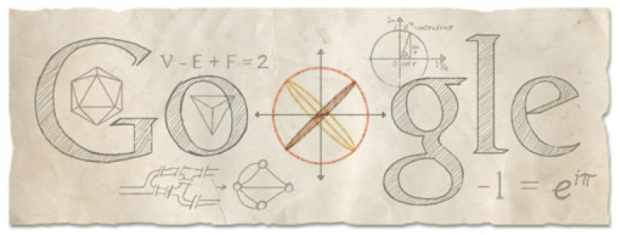
\includegraphics[width=\textwidth]{pagerank}
\end{minipage}

\pagebreak
\section{Exponentiële functies}

\subsection{Inleiding}

Bij Isa's geboorte stelt haar grootmoeder, een wiskundige, aan de moeder van Isa, ook een wiskundige, twee plannen voor om haar jaarlijks een beetje spaargeld te schenken tot ze 18 jaar is.

\begin{description}
  \item[Plan A] Isa krijgt bij haar geboorte en bij elke verjaardag 1000 euro. Daarbij komt nog dat ze bij elke verjaardag een opslag krijgt van 100 euro.
  \item[Plan B] Isa krijgt bij de geboorte 1 euro en bij elke verjaardag wordt het bedrag verdubbeld.
\end{description}

\begin{oefening}
Welk plan zou jij kiezen?
\arules{1}
\end{oefening}

\begin{oefening}
Maak een tabel waarbij je de schenkingen uitzet in functie van de leeftijd:
\begin{center}
  \renewcommand{\arraystretch}{1.1}
  \begin{tabular}{c|c|c}
  \arule{3cm}&\arule{3cm}&\arule{3cm}\\
  \hline
  \arule{2cm}&\arule{2cm}&\arule{2cm}\\    
  \arule{2cm}&\arule{2cm}&\arule{2cm}\\    
  \arule{2cm}&\arule{2cm}&\arule{2cm}\\    
  \arule{2cm}&\arule{2cm}&\arule{2cm}\\    
  \arule{2cm}&\arule{2cm}&\arule{2cm}\\    
  \arule{2cm}&\arule{2cm}&\arule{2cm}\\    
  \arule{2cm}&\arule{2cm}&\arule{2cm}\\    
  \arule{2cm}&\arule{2cm}&\arule{2cm}\\    
  \arule{2cm}&\arule{2cm}&\arule{2cm}\\    
  \arule{2cm}&\arule{2cm}&\arule{2cm}\\    
  \arule{2cm}&\arule{2cm}&\arule{2cm}\\    
  \arule{2cm}&\arule{2cm}&\arule{2cm}\\    
  \arule{2cm}&\arule{2cm}&\arule{2cm}\\    
  \arule{2cm}&\arule{2cm}&\arule{2cm}\\    
  \arule{2cm}&\arule{2cm}&\arule{2cm}\\    
  \arule{2cm}&\arule{2cm}&\arule{2cm}\\    
  \arule{2cm}&\arule{2cm}&\arule{2cm}\\    
  \arule{2cm}&\arule{2cm}&\arule{2cm}\\    
  \arule{2cm}&\arule{2cm}&\arule{2cm}\\    
  \end{tabular}
\end{center}
\end{oefening}

\begin{oefening}
Zoek voor elk het bijhorende functievoorschrift. Voer dit dan in op je \zrm{ZRM} en controleer bovenstaande tabel. De tabel functionaliteit op je rekenmachine gebruik je als volgt: \zrm{MODE}\zrm{4:TABLE}. Om terug naar de normale rekenmodus te gaan met je rekenmachine kies je \zrm{MODE}\zrm{4:COMP}. Teken dan ook de grafiek.\\

\begin{minipage}{0.5\textwidth}
  \centering
  {\bf Plan A}
  $$y=\arule{3cm}$$
  \assenstelsel[0.7]{-1}{8}{-1}{20}
\end{minipage}
\begin{minipage}{0.5\textwidth}
  \centering
  {\bf Plan B}
  $$y=\arule{3cm}$$
  \assenstelsel[0.7]{-1}{8}{-1}{20}
\end{minipage}
\end{oefening}

De grafiek uit plan A herkennen we als punten gelegen op een rechte. Dit komt ook overéén met het functievoorschrift bij plan A (\arule{5cm} of \arule{5cm}). De grafiek uit plan B bestaat uit punten gelegen op een snel stijgende kromme. Een kromme van deze vorm zullen we een {\bf exponentiële kromme} noemen en horen bij {\bf exponentiële functies}. De eigenschappen van deze functies zullen we in dit hoofdstuk bestuderen.

\subsection{Definitie van een exponentiële functie}

\paragraph*{Definitie}
\begin{mdframed}
Een {\bf exponentiële functie} is een functie
$$f:\mathbb{R}\to\mathbb{R}: x\mapsto a^x$$
met $a\in\mathbb{R}^+\backslash\{0,1\}$.
\end{mdframed}

Het getal $a$ wordt het {\bf grondtal} van de exponentiële functie genoemd, de onbepaalde $x$ treed op als de {\bf exponent}.

\begin{oefening}
In de definitie worden drie eisen opgelegd aan het grondtal $a$, welke en waarom?
\begin{itemize}
  \item \arulefill\arules{1}
  \item \arulefill\arules{1}
  \item \arulefill\arules{1}
\end{itemize}
\end{oefening}

\begin{oefening}
Er zijn drie manieren waarop we een functievoorschrift kunnen geven, geef ze alle drie:
\begin{itemize}
  \itemsep1em
  \item $f:\mathbb{R}\to\mathbb{R}: x\mapsto 3^x$
  \item \arulefill
  \item \arulefill
\end{itemize}
\end{oefening}

\begin{oefening}
Er zijn drie manieren waarop we een functievoorschrift kunnen geven, geef ze alle drie:
\begin{itemize}
  \itemsep1em
  \item \arulefill
  \item $f(x)=(0.5)^x$
  \item \arulefill
\end{itemize}
\end{oefening}


\subsection{Grafiek van een exponentiële functie}
\vspace*{-1cm}

\begin{oefening}
Bespreek de exponentiële functie $f:\mathbb{R}\to\mathbb{R}: x\mapsto 2^x$
\paragraph*{Functievoorschrift:}
\begin{center}
\visgraad{12cm}
\end{center}
\paragraph*{Grafiek:}
\begin{center}
\vspace*{-0.5cm}
\assenstelsel{-4}{5}{-1}{9}
\end{center}
\paragraph*{Domein en bereik:} \arulefill
\paragraph*{Tekenverloop:}
\begin{center}
\vspace*{-0.5cm}
\visgraad{5cm}
\end{center}
\paragraph*{Stijgen en dalen:}
\begin{center}
\vspace*{-0.5cm}
\visgraad{5cm}
\end{center}
\paragraph*{Limieten:} \arulefill
\paragraph*{Asymptoten:} \arulefill
\end{oefening}

\begin{oefening}
Bespreek de exponentiële functie $f:\mathbb{R}\to\mathbb{R}: x\mapsto \left(\dfrac{1}{2}\right)^x$
\paragraph*{Functievoorschrift:}
\begin{center}
\visgraad{12cm}
\end{center}
\paragraph*{Grafiek:}
\begin{center}
\vspace*{-0.5cm}
\assenstelsel{-4}{5}{-1}{9}
\end{center}
\paragraph*{Domein en bereik:} \arulefill
\paragraph*{Tekenverloop:}
\begin{center}
\vspace*{-0.5cm}
\visgraad{5cm}
\end{center}
\paragraph*{Stijgen en dalen:}
\begin{center}
\vspace*{-0.5cm}
\visgraad{5cm}
\end{center}
\paragraph*{Limieten:} \arulefill
\paragraph*{Asymptoten:} \arulefill
\end{oefening}

\subsection{Eigenschappen van exponentiële functies}

Gezien de vorige twee oefeningen kunnen we twee gevallen onderscheiden, deze waarbij ons grondtal $a>1$ (a groter dan één) is en deze waarbij ons grondtal $0<a<1$ (a tussen nul en één) is.

In de volgende twee assenstelsels worden nog een aantal extra voorbeelden gegeven, waarbij goed de afhankelijkheid van het grondtal $a$ duidelijk wordt.

\begin{minipage}{0.5\textwidth}
$$a>1$$
\begin{center}
\begin{tikzpicture}
\begin{axis}[grid=both,
          xmax=5,ymax=10,
          axis lines=middle,
          restrict y to domain=-1:12,
          enlargelimits]
\addplot[line width=1.2pt]  {pow(2,x)} node[above]{$2^x$};
\addplot[line width=1.2pt]  {pow(3,x)} node[above]{$3^x$};
\addplot[line width=1.2pt]  {pow(1.5,x)} node[above]{$(1.5)^x$};
\end{axis}
\end{tikzpicture}
\end{center}
\end{minipage}
\begin{minipage}{0.5\textwidth}
$$0<a<1$$
\begin{center}
\begin{tikzpicture}
\begin{axis}[grid=both,
          xmax=5,ymax=10,
          axis lines=middle,
          restrict y to domain=-1:12,
          enlargelimits]
\addplot[line width=1.2pt]  {pow(0.5,x)} node[pos=0, above]{$0.5^x$};
\addplot[line width=1.2pt]  {pow(0.25,x)} node[pos=0, above]{$0.25^x$};
\addplot[line width=1.2pt]  {pow(0.75,x)} node[pos=0, above]{$(0.75)^x$};
\end{axis}
\end{tikzpicture}
\end{center}
\end{minipage}

\begin{oefening}
Bepaal zelf de eigenschappen: domein, bereik, bijzondere punten, dalen\&stijgen, limieten en asymptoten:
\arules{13}
\end{oefening}

\begin{oefening}
Gebruik {\em Geogebra} om de exponentiële functie $f(x)=a^x$ te plotten, waarbij $a$ een parameter is die je instelt via een schuifknop. Volg hierbij de volgende instructies:
\begin{itemize}
  \item Download of start geogebra vanuit \url{http://geogebra.org/}.
  \item Het geogebravenster bevat bovenaan de {\em menubar}, daaronder de {\em iconen}, een {\em algebravenster} en een {\em tekenvenster}. Helemaal onderaan hebben we de {\em invoer} waar je commando's kan geven aan geogebra en waarbinnen je objecten kan definiëren.
  \item
  \begin{minipage}[t]{0.5\textwidth}
  \vspace{0pt}
  Zoek binnen de iconen naar de knop om een {\em schuifknop} te definiëren, click hier op en plaats deze op een willekeurig positie in het tekenvenster.
  \end{minipage}
  \begin{minipage}[t]{0.5\textwidth}
  \vspace{0pt}
  \begin{center}
    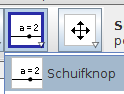
\includegraphics{gg_schuifknop_icoon}
  \end{center}
  \end{minipage}
  \item
  \begin{minipage}[t]{0.3\textwidth}
  \vspace{0pt}
  De eigenschappen van de schuifknop moeten als volgt zijn:
  \begin{itemize}
    \item Naam: \verb#a#
    \item Interval: $]0,3]$ met stapgrootte $0.1$
  \end{itemize}
  \end{minipage}
  \begin{minipage}[t]{0.7\textwidth}
  \vspace{0pt}
  \begin{center}
    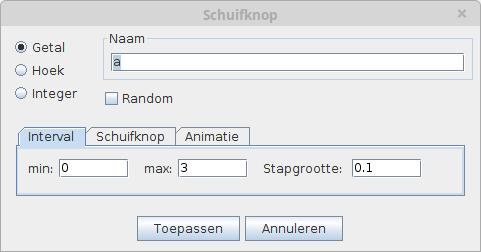
\includegraphics[width=0.7\textwidth]{gg_schuifknop_eigenschappen}
  \end{center}
  \end{minipage}
  \item 
  \begin{minipage}[t]{0.6\textwidth}
  \vspace{0pt}
  Typ \verb#f(x)=a^x# in de invoer om de functie te definiëren. Het symbool '\verb#^#' staat voor 'tot de macht'.
  \end{minipage}
  \begin{minipage}[t]{0.4\textwidth}
  \vspace{0pt}
  \begin{center}
    
\includegraphics{gg_invoer_funct}
  \end{center}
  \end{minipage}
  \item Gebruik de schuifknop nu om de exponentiële functie te plotten met verschillende waarden voor $a$.
\end{itemize}
\begin{center}
  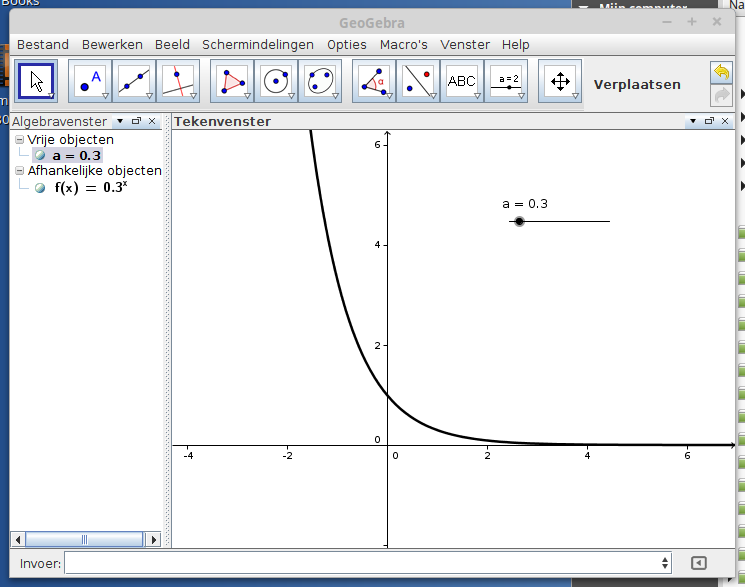
\includegraphics[width=0.5\textwidth]{gg_afgewerkt}
\end{center}
\end{oefening}

\begin{oefening}
Gebruik {\em Geogebra} om de exponentiële functie $f(x)=a^{x-b}+c$ te plotten, waarbij $a\in]0,3]$, $b\in[-3,3]$ en $c\in[-3,3]$ parameters zijn die je instelt via schuifknoppen. Gebruik haakjes om aan geogebra duidelijk te maken dat de exponent $x-b$ samen hoort.
\end{oefening}

\begin{oefening}
Teken de grafiek van, maak daarvoor steeds een functiewaardentabel in $[-5,5]$.
\begin{exlist}{2}
  \item $y=4^x$
  \item $y=\left(\dfrac{1}{4}\right)^x$
  \item $y=\left(\dfrac{3}{2}\right)^x$
  \item $y=3^x-1$
  \item $y=2^{x-3}$
  \item $y=4\cdot \left(\dfrac{1}{2}\right)^x$
\end{exlist}
\end{oefening}

\begin{oefening}
Maak de grafiek van de volgende exponentiële functies
\begin{multicols}{3}
\begin{enumerate}[(a)]
  \item $f(x)=10^x$
  \item $f(x)=0.5^x$
  \item $f(x)=e^x$
\end{enumerate}
\end{multicols}
Het getal $e$, het getal van Euler, is een constante die je op je rekentoestel vindt. Druk \zrm{SHIFT} \zrm{$e^\blacksquare$} en dan de exponent.
\end{oefening}

\begin{oefening}
Gegeven de grafiek van de exponentiële functie $f(x)=a^x$. Bepaal telkens de waarde van $a$.
\begin{multicols}{3}
\begin{enumerate}[(a)]
  \item\raisebox{-3cm}{
\definecolor{cqcqcq}{rgb}{0.75,0.75,0.75}
\begin{tikzpicture}[line cap=round,line join=round,>=triangle 45,x=1.0cm,y=1.0cm]
\draw [color=cqcqcq,dash pattern=on 1pt off 1pt, xstep=0.5cm,ystep=0.5cm] (-1.06,-0.3) grid (2.68,2.58);
\draw[->,color=black] (-1.06,0) -- (2.68,0);
\foreach \x in {1,2}
\draw[shift={(\x,0)},color=black] (0pt,2pt) -- (0pt,-2pt) node[below] {\footnotesize $\x$};
\draw[->,color=black] (0,-0.3) -- (0,2.58);
\foreach \y in {1,2}
\draw[shift={(0,\y)},color=black] (2pt,0pt) -- (-2pt,0pt) node[left] {\footnotesize $\y$};
\draw[color=black] (0pt,-10pt) node[right] {\footnotesize $0$};
\clip(-1.06,-0.3) rectangle (2.68,2.58);
\draw(2.02,-1.54) -- (2.95,-1.54);
\draw[line width=1.6pt, smooth,samples=100,domain=-1.06:2.68] plot(\x,{exp(ln(0.25)*\x});
\end{tikzpicture}
}
  \item\raisebox{-3cm}{
\definecolor{cqcqcq}{rgb}{0.75,0.75,0.75}
\begin{tikzpicture}[line cap=round,line join=round,>=triangle 45,x=1.0cm,y=1.0cm]
\draw [color=cqcqcq,dash pattern=on 1pt off 1pt, xstep=0.5cm,ystep=0.5cm] (-1.06,-0.3) grid (2.68,2.58);
\draw[->,color=black] (-1.06,0) -- (2.68,0);
\foreach \x in {1,2}
\draw[shift={(\x,0)},color=black] (0pt,2pt) -- (0pt,-2pt) node[below] {\footnotesize $\x$};
\draw[->,color=black] (0,-0.3) -- (0,2.58);
\foreach \y in {1,2}
\draw[shift={(0,\y)},color=black] (2pt,0pt) -- (-2pt,0pt) node[left] {\footnotesize $\y$};
\draw[color=black] (0pt,-10pt) node[right] {\footnotesize $0$};
\clip(-1.06,-0.3) rectangle (2.68,2.58);
\draw(2.02,-1.54) -- (2.95,-1.54);
\draw[line width=1.6pt, smooth,samples=100,domain=-1.06:2.68] plot(\x,{exp(ln(1.5)*\x});
\end{tikzpicture}
}
  \item\raisebox{-3cm}{
\definecolor{cqcqcq}{rgb}{0.75,0.75,0.75}
\begin{tikzpicture}[line cap=round,line join=round,>=triangle 45,x=1.0cm,y=1.0cm]
\draw [color=cqcqcq,dash pattern=on 1pt off 1pt, xstep=0.5cm,ystep=0.5cm] (-1.06,-0.3) grid (2.68,2.58);
\draw[->,color=black] (-1.06,0) -- (2.68,0);
\foreach \x in {1,2}
\draw[shift={(\x,0)},color=black] (0pt,2pt) -- (0pt,-2pt) node[below] {\footnotesize $\x$};
\draw[->,color=black] (0,-0.3) -- (0,2.58);
\foreach \y in {1,2}
\draw[shift={(0,\y)},color=black] (2pt,0pt) -- (-2pt,0pt) node[left] {\footnotesize $\y$};
\draw[color=black] (0pt,-10pt) node[right] {\footnotesize $0$};
\clip(-1.06,-0.3) rectangle (2.68,2.58);
\draw(2.02,-1.54) -- (2.95,-1.54);
\draw[line width=1.6pt, smooth,samples=100,domain=-1.06:2.68] plot(\x,{exp(ln(2)*\x});
\end{tikzpicture}
}
\end{enumerate}
\end{multicols}
\end{oefening}

\begin{oefening}
Schets de volgende functies, probeer dit te doen zonder een functiewaardentabel te maken.
\begin{multicols}{3}
\begin{enumerate}[(a)]
  \item $f(x)=2^x+2.5$
  \item $f(x)=2^{x-1.5}$
  \item $f(x)=0.5^{2x}$
\end{enumerate}
\end{multicols}
Hint: Probeer (c) eerst in de vorm $f(x)=a^x$ te brengen.
\end{oefening}

\begin{oefening}
Bepaal de volgende limieten:
\begin{multicols}{3}
\begin{enumerate}[(a)]
  \item $\displaystyle\lim_{x\to+\infty}3^x$
  \item $\displaystyle\lim_{x\to-\infty}3^x$
  \item $\displaystyle\lim_{x\to0}3^x$
  \item $\displaystyle\lim_{x\to1}3^x$
  \item $\displaystyle\lim_{x\to+\infty}0.01^x$
  \item $\displaystyle\lim_{x\to-\infty}1.1^x$
  \item $\displaystyle\lim_{x\to-\infty}0.99^x$
  \item $\displaystyle\lim_{x\to+\infty}0.5^x+1.5$
  \item $\displaystyle\lim_{x\to+\infty}2^{-x}$
\end{enumerate}
\end{multicols}
\end{oefening}

\begin{oefening}*
Gegeven de grafiek van $f(x)=e^x$, schets de grafieken van de functies met voorschriften:
\begin{multicols}{3}
\begin{enumerate}[(a)]
  \item $g(x)=f(x)-1$
  \item $g(x)=-f(x)$
  \item $g(x)=2\cdot f(x)$
  \item $g(x)=-2\cdot f(x)$
  \item $g(x)=f(x-2.5)$
  \item $g(x)=f(-x)$
\end{enumerate}
\end{multicols}
\end{oefening}

\begin{oefening}*
Een functie met voorschrift $y=k\cdot a^x$ gaat door $P(-1,2)$ en $Q(2,\dfrac{125}{32})$. Bepaal $a$ en $k$.
\end{oefening}

\pagebreak

\section{Toepassingen op exponentiële functies}

\subsection{Exponentiële groei}

\begin{oefening}
Op het tijdstip $t=0$ bevat een bacteriënkolonie $N_0=400$ bacteriën. Elk uur groeit het aantal met $p\%=5\%$. Stel een formule op die het aantal bacteriën $N$ geeft na $t$ uur. Gebruik die formule om het aantal bacteriën te vinden na $24$ uur.
\end{oefening}

\paragraph*{Oplossing}
We gaan het probleem opsplitsen. We zullen eerst onderzoeken hoeveel bacteriën er zullen zijn na één uur, dan na twee uur, dan na drie uur, \ldots

\begin{itemize}
  \item Na 1 uur:
  \begin{itemize}
    \item Bij aanvang: \arule{4cm}
    \item Aangroei: \arule{4cm}
    \item Na één uur: \arule{4cm}
  \end{itemize}
  Herschrijven geeft ons: \arules{2}\\
  Dus $400$ met $5\%$ vermeerderen = \arulefill
  \item Na 2 uur:
  \begin{itemize}
    \item Bij aanvang: \arule{4cm}
    \item Aangroei: \arule{4cm}
    \item Na één uur: \arule{4cm}
  \end{itemize}
  Herschrijven geeft ons: \arules{2}\\
  Dus $420$ met $5\%$ vermeerderen = \arulefill
  Maar $420$ konden we reeds bekomen uit onze oorspronkelijke aantal bacteriën: \arules{2}\\
  Dus $400$ tweemaal met $5\%$ vermeerderen = \arulefill
  \item Na 3 uur:
  \begin{itemize}
    \item Bij aanvang: \arule{4cm}
    \item Aangroei: \arule{4cm}
    \item Na één uur: \arule{4cm}
  \end{itemize}
  Herschrijven geeft ons: \arules{2}\\
  Dus $441$ met $5\%$ vermeerderen = \arulefill
  Maar $441$ konden we reeds bekomen uit onze oorspronkelijke aantal bacteriën: \arules{2}\\
  Dus $400$ driemaal met $5\%$ vermeerderen = \arulefill
  \item Na 4 uur: \arulefill
  \item Aantal bacteriën $N$ na $t$ uur: \arulefill
  \item Toepassen van de formule voor na $24$ uur: \arulefill
\end{itemize}

\begin{oefening}
Veronderstel dat de populatie van een bepaald land jaarlijks aangroeit met $2\%$. Als het land momenteel 3 miljoen inwoners telt, wat zal dan de populatie zijn over 10 jaar?
\end{oefening}

\paragraph*{Exponentiële groei}

\begin{mdframed}
Als $N_0$ de {\bf beginwaarde} is en $p\%$ het {\bf groeipercentage} is, dan wordt de aangroei na {\bf tijd} $t$ gegeven door
$$N=N_0\cdot\left(1+\dfrac{p}{100}\right)^t$$
en hierin wordt $1+\dfrac{p}{100}$ de {\bf groeifactor} genoemd.
\end{mdframed}

De groeifactor zullen we meestal kort kunnen schrijven, als het groeipercentage bijvoorbeeld $15\%$ is, dan wordt de groeifactor, door invullen van $p$ en te vereenvoudigen, $1.15$.

\begin{oefening}
Geef een vijftal voorbeelden uit de natuur of het dagelijks leven waar je denkt van exponentiële groei tegen te komen.
\arules{1}
\end{oefening}

\subsection{Exponentiële daling}

We kunnen de formule van exponentiële groei ook gaan toepassen op problemen waarbij er op elk tijdstip een vermindering is i.p.v. een vermeerdering. Beschouw volgende oefening:

\begin{oefening}
Elk jaar sponsort de lokale tennisclub van Avelgem een tornooi. Er wordt begonnen met 128 deelnemers. Bij elke ronde wordt de helft van de deelnemers geëlimineerd. Hoeveel deelnemers blijven er over na 5 rondes?

\paragraph*{Oplossing}
\begin{itemize}
  \itemsep1em
  \item Gebruik een tabel:
  \begin{center}
    \begin{tabular}{c|r|r|r|r|r|r}
      Ronde & start & 1ste & 2de & 3de & 4de & 5de\\
      \hline
      Spelers & 128 & \arule{1cm} & \arule{1cm} & \arule{1cm} & \arule{1cm} & \arule{1cm}
    \end{tabular}
  \end{center}
  \item Gebruik de formule:\\
  $$N=N_0\cdot\left(1+\dfrac{p}{100}\right)^t$$\\
  Met $N_0 = \arule{2cm}$, $t=\arule{2cm}$ en $p=\arule{2cm}$:
  $$N=\arule{5cm}$$
\end{itemize}
\end{oefening}

\subsection{Halveringstijd}

In de vorige oefening werden het aantal deelnemers elke ronde gehalveerd. In veel problemen met de natuur is de tijd nodig om 'iets' te halveren belangrijk, daarom volgende definitie:\\

\begin{mdframed}
De {\bf halveringstijd} is de tijd nodig om het aantal deeltjes te halveren.
\end{mdframed}

\paragraph*{Voorbeeld}
De pesticide {\em DDT} werd vroeger vaak gebruikt in de landbouw. Snel werd echter duidelijk dat DDT niet enkel onkruid verdelgde, maar ook giftig was voor dieren. Er wordt ondertussen ook aangenomen dat DDT bepaalde kankers veroorzaakt. De halveringstijd van DDT is 15 jaar. Dit wil zeggen dat als er 100 gram DDT aanwezig is op een akker van een boer, dat de DDT dan in de loop van 15 jaar afbreekt tot 50 gram. De volgende 15 jaar zal de DDT op de akker afbreken tot 25 gram, enz...

\begin{oefening}
Plot de functie die het verloop van 100 gram DDT  weergeeft over een periode van 100 jaar.
\begin{center}
\visgraad{12cm}
\assenstelsel{-1}{12}{-1}{12}
\end{center}
\end{oefening}

Het is mogelijk om onmiddellijk de hoeveelheid DDT uit te rekenen na 100 jaar. We maken hiervoor gebruik van de volgende formule:

\paragraph*{Halveringsformule}
\begin{mdframed}
Als $N_0$ het aantal deeltijdjes is op tijdstip $t=0$ en $T$ is de {\bf halveringstijd}, dan wordt het aantal deeltjes op tijdstip $t$ gegeven door
$$N=N_0\cdot2^{-\frac{t}{T}}\;.$$
$N_0$ wordt ook nog de {\bf beginwaarde} genoemd. $t$ en $T$ moeten altijd in dezelfde eenheid gegeven worden.
\end{mdframed}

\begin{oefening}
Maak gebruik van de halveringsformule
$$N=N_0\cdot2^{-\frac{t}{T}}$$
om te weten hoeveel gram van de 100 gram DDT er nog aanwezig zal zijn na 100 jaar.
\paragraph*{Oplossing}
\begin{itemize}
  \itemsep1em
  \item $N_0=\arule{4cm}$
  \item $t = \arule{4cm}$
  \item $T = \arule{4cm}$
  \item $N = $ \arulefill
\end{itemize}
\end{oefening}

\begin{oefening}
Elke plant bevat de radioactieve koolstofisotoop $\ce{C14}$. Zolang de plant leeft, blijft de aanwezigheid van die isotoop constant. Wanneer de plant sterft, dan daalt de aanwezigheid van de koolstofisotoop.
\begin{enumerate}[(a)]
  \item Wat is de halveringstijd van koolstof-14 (\ce{C14})?
  \item Hoeveel percent van de koolstofisotoop \ce{C14} blijft er over in een houten beeldje dat 1500 jaar geleden van het hout van een pas gehakte boom werd gemaakt?
\end{enumerate}
\end{oefening}

\begin{oefening}
Geef een vijftal voorbeelden uit de natuur of het dagelijks leven waar je denkt exponentiële daling tegen te komen.
\arules{1}
\end{oefening}

\subsection{Oefeningen}

\begin{oefening}
We beleggen 10000 euro op de bank. De bank geeft ons een interest van $2.5\%$ (interest + getrouwheidspremie).
\begin{enumerate}[(a)]
  \item Geef de groeiformule.
  \item Hoeveel zal er op onze rekening staan na 1 jaar?
  \item Hoeveel zal er op onze rekening staan na 25 jaar?
  \item Hoe lang moeten we wachten tot ons geld is verdubbeld?
\end{enumerate}
\end{oefening}

\begin{oefening}
In een bepaald land neemt de bevolking jaarlijks met $2\%$ toe. Momenteel wonen er 500 000 mensen. Hoeveel inwoners zijn er over 10 jaar?
\end{oefening}

\begin{oefening} % source: Jennenkens p246
In een bacteriëncultuur, met initieel 100 bacteriën, verdubbelt het aantal bacteriën elke maand. We nomen 2 de {\em groeifactor} per maand en één maand de {\em verdubbelingstijd}.
\begin{enumerate}[(a)]
  \item Hoeveel bacteriën zijn er na 3 maanden?
  \item Hoeveel bacteriën zijn er na 1 jaar?
  \item Bereken de groeifactor per week.
\end{enumerate}
\end{oefening}

\begin{oefening} % source: Jennenkens p246
Een tropisch land haalt voor zijn watervoorziening aan de noordpool een ijsberg van 10 miljoen $m^3$. Dagelijks smelt $5\%$ weg.
\begin{enumerate}[(a)]
  \item Geef een formule die de inhoud $I$ van de ijsberg geeft na $t$ dagen.
  \item De vaart duurt 10 dagen. Blijft er meer dan de helft van de ijsberg over?
\end{enumerate}
\end{oefening}

\begin{oefening} % source: Jennenkens p246
Bereken met de formule $N=N_0\cdot 2^{-t/T}$ hoeveel percent van de deeltjes nog aanwezig is na de gegeven tijd voor:\\
\begin{tabular}{clll}
(a) & \ce{Pb214} (lood) & T=27 min & na 1 uur\\    
(b) & \ce{Rn222} (radon) & T=3.8 dagen & na 10 dagen\\
(c) & \ce{Th234} (thallium) & T=24 dagen & na 90 dagen\\
(d) & \ce{Po210} (polonium) & T=140 dagen & na 1 jaar
\end{tabular}
\end{oefening}

\begin{oefening}
Licht radioactief afval met een halveringstijd van 30 jaar wordt gedurende 300 jaar in tonnen bewaard. Hoeveel percent van het oorspronkelijke aantal radioactieve elementen blijft er dan nog over?
\end{oefening}

\begin{center}
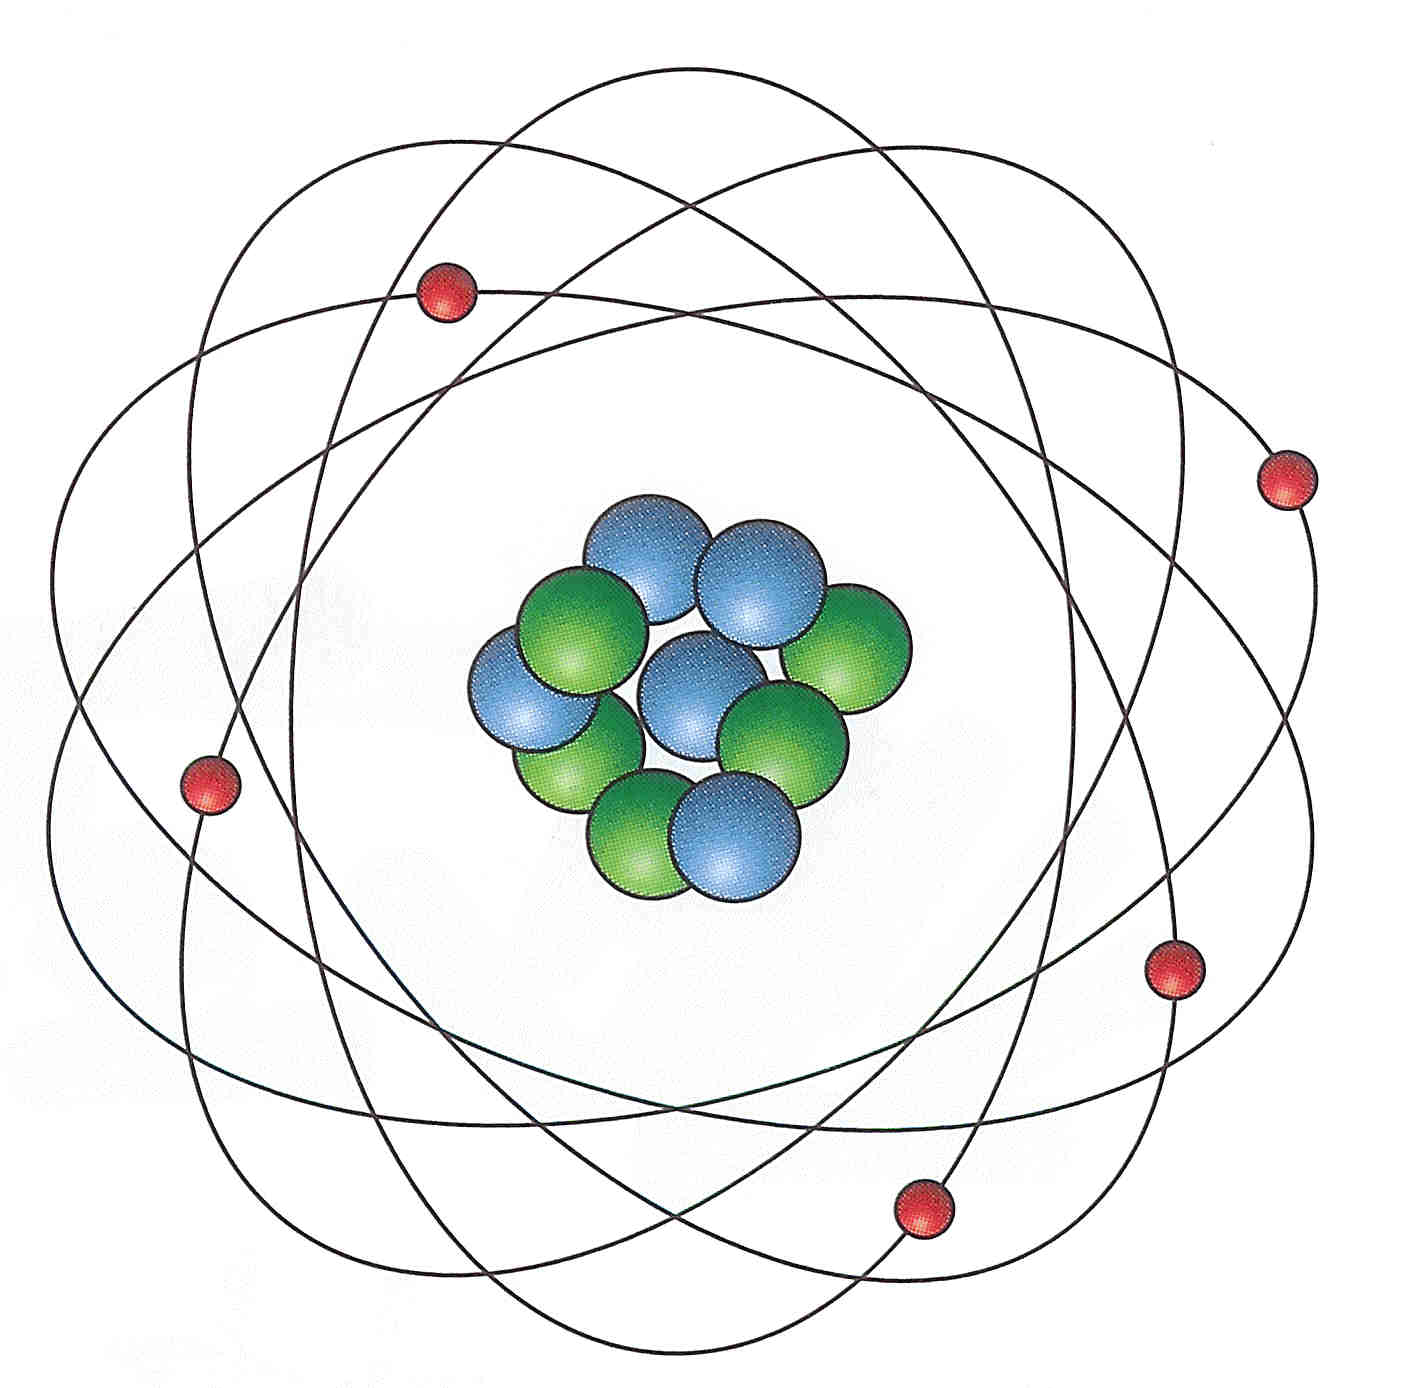
\includegraphics[width=0.5\textwidth]{atoom_boor}
\end{center}

%%%%%%%%%%%%%%%%%%%%%%%%%%%%%%%%%%%%%%%%%%%%%%%%%%%%%%%%%%%%%%%%%%%%%%
\end{document}




\begin{minipage}[c]{0.4\textwidth}
\end{minipage}
\begin{minipage}[c]{0.6\textwidth}
\dotlines{10}
\end{minipage}




















